\documentclass{standalone}

\usepackage{circuitikz}

\begin{document}

% INT_AY21_L30_Fig02_Missing_curr_volt.png

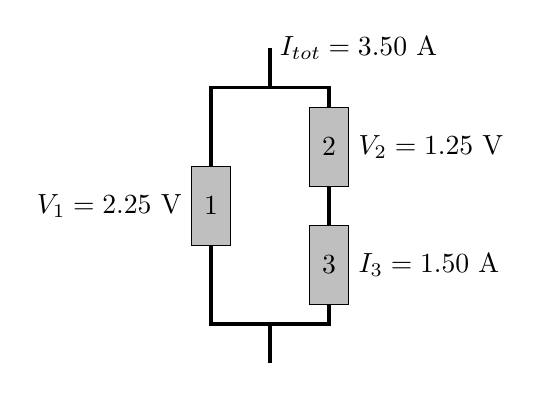
\begin{tikzpicture}

	% Circuit elements
	
	\begin{scope}[gray!50, draw = black]

		\filldraw (-1, -0.5) rectangle (-0.5, 0.5);
		\filldraw (1, 1.25) rectangle (0.5, 0.25);
		\filldraw (1, -1.25) rectangle (0.5, -0.25);
	
	\end{scope}
	
	\node at (-0.75, 0) {1};
	\node at (0.75, 0.75) {2};
	\node at (0.75, -0.75) {3};
	
	% Wires
	
	\begin{scope}[very thick]
		
		\draw (0, 1.5) -- (0, 2);
		\draw (-0.75, 0.5) -- (-0.75, 1.5) -- (0.75, 1.5) -- (0.75, 1.25);
		\draw (0.75, 0.25) -- (0.75, -0.25);
		\draw (-0.75, -0.5) -- (-0.75, -1.5) -- (0.75, -1.5) -- (0.75, -1.25);
		\draw (0, -1.5) -- (0, -2);
	
	\end{scope}
	
	% Given currents, voltages
	
	\node [right] at (0, 2) {$I_{tot} = 3.50$ A};
	\node [left] at (-1, 0) {$V_1 = 2.25$ V};
	\node [right] at (1, 0.75) {$V_2 = 1.25$ V};
	\node [right] at (1, -0.75) {$I_3 = 1.50$ A};

\end{tikzpicture}

\end{document}